\chapter{Câu hỏi ôn tập}
\hideall{
\setcounter{section}{0}
\begin{center}
	\textbf{\large BẢNG ĐÁP ÁN}
\end{center}
\section{Câu trắc nghiệm nhiều phương án lựa chọn}
\inputansbox{10}{ans/Y24-VN12-PH-C2-TN}
\section{Câu trắc nghiệm đúng sai}
\inputansbox[2]{2}{ans/Y24-VN12-PH-C2-TF}
\section{Câu trắc nghiệm trả lời ngắn}
\inputansbox[3]{6}{ans/Y24-VN12-PH-C2-TL}
}
\setcounter{section}{0}
\section{Câu trắc nghiệm nhiều phương án lựa chọn}
\textit{Thí sinh trả lời từ câu 1 đến câu 18. Mỗi câu thí sinh chọn một phương án}
\setcounter{ex}{0}
\Opensolutionfile{ans}[ans/Y24-VN12-PH-C2-TN]
% ===================================================================
\begin{ex}
	heo thuyết động học phân tử chất khí, áp suất của một khối lượng khí nhất định chứa trong một bình có thể tích xác định giảm là vì
	\begin{enumerate}[label=(\arabic*)]
		\item tốc độ trung bình của các phân tử khí giảm.
		\item các phân tử khí va chạm với thành bình chứa ít thường xuyên hơn.
		\item nhiệt độ của chất khí giảm.
	\end{enumerate}
	Nhận định nào đúng?
	\choice
	{Chỉ (2)}
	{(1) và (2)}
	{(1) và (3)}
	{\True (1), (2) và (3)}
	\loigiai{}
\end{ex}
% ===================================================================
\begin{ex}
	Khi một chất khí trong một bình kín bị đun nóng, áp suất chất khí tăng lên. Phát biểu nào sau đây giải thích đúng hiện tượng này?
	\choice
	{Các phân tử khí dãn nở và trở nên nặng hơn, vì thế chúng va chạm nhau mạnh hơn}
	{Các phân tử khí có ít không gian chuyển động hơn, nên chúng va chạm nhau thường xuyên hơn}
	{Các phân tử khí va chạm vào thành bình mạnh hơn nhưng ít thường xuyên hơn}
	{\True Các phân tử khí chuyển động nhanh hơn, vì thế chúng va chạm với thành bình thường xuyên hơn}
	\loigiai{}
\end{ex}
% ===================================================================
\begin{ex}
	Một khối khí nhất định được chứa trong một xilanh kín với một pit-tông động. Ban đầu, khối khí ở áp suất $p_1$ và có thể tích $V_1$. Nhiệt độ được giữ không đổi. Pit-tông dịch chuyển sao cho áp suất trở thành $p_2$ và thể tích trở thành $V_2$. Chỉ ra biểu thức đúng.
	\choice
	{$\dfrac{p_1}{V_1}=\dfrac{p_2}{V_2}$}
	{$\dfrac{p_1}{p_2}=\dfrac{V_1}{V_2}$}
	{\True $p_1 V_1=p_2 V_2$}
	{$p_1 V_2=p_2 V_1$}
	\loigiai{}
\end{ex}
% ===================================================================
\begin{ex}
	Trong hệ tọa độ $(p, V)$, đường biểu diễn quá trình đẳng nhiệt của một khối khí lí tưởng có dạng
	\choice
	{một đường thẳng đứng}
	{một phần của elip}
	{một phần của parabol}
	{\True một phần của hyperbol}
	\loigiai{}
\end{ex}
% ===================================================================
\begin{ex}
	\immini{
	Hình bên mô tả một khối khí bị giữ bên trong một xilanh bởi một pit-tông động. Thể tích của khối khí là $\SI{120}{\centi\meter^3}$ và áp suất của khối khí là $p$. Từ từ di chuyển pit-tông sang trái sao cho thể tích khối khí giảm còn $\SI{30}{\centi\meter^3}$. Nhiệt độ của khối khí không đổi. Áp suất mới của khối khí trong xilanh là bao nhiêu?
	}
	{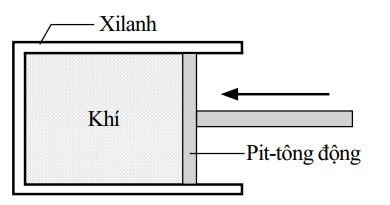
\includegraphics[width=0.5\linewidth]{../figs/G12C2-1}}
	\choice
	{$\dfrac{p}{4}$}
	{$\dfrac{p}{2}$}
	{$p$}
	{\True $4 p$}
	\loigiai{}
\end{ex}
% ===================================================================
\begin{ex}
	Có $\SI{400}{\centi\meter^3}$ khí lí tưởng ở $\SI{0}{\celsius}$. Nếu được đun nóng ở áp suất không đổi để nhiệt độ tăng lên đến $\SI{10}{\celsius}$ thì khối khí sẽ chiếm thể tích
	\choice
	{\True $\SI{415}{\centi\meter^3}$}
	{$\SI{283}{\centi\meter^3}$}
	{$\SI{278}{\centi\meter^3}$}
	{$\SI{493}{\centi\meter^3}$}
	\loigiai{}
\end{ex}
% ===================================================================
\begin{ex}
	Hai bình có thể tích bằng nhau chứa cùng một loại khí. Áp suất và nhiệt độ tuyệt đối của khí trong mỗi bình lần lượt là $p_1$ và $p_2, T_1$ và $T_2$. Hai bình được nối thông với nhau và chất khí đạt tới áp suất chung $p$ và nhiệt độ tuyệt đối chung $T$. Chỉ ra biểu thức đúng.
	\choice
	{$\dfrac{p}{T}=\dfrac{p_1}{T_1}+\dfrac{p_2}{T_2}$}
	{\True $\dfrac{p}{T}=\dfrac{1}{2}\left(\dfrac{p_1}{T_1}+\dfrac{p_2}{T_2}\right)$}
	{$\dfrac{p}{T}=\dfrac{p_1 T_2+p_2 T_1}{2\left(T_1+T_2\right)}$}
	{$\dfrac{p}{T}=\dfrac{p_1+p_2}{T_1+T_2}$}
	\loigiai{}
\end{ex}
% ===================================================================
\begin{ex}
	Giả sử một khối khí ban đầu ở nhiệt độ chuẩn và khối khí chịu sự biến đổi sao cho áp suất của nó tăng gấp bốn lần còn nhiệt độ tuyệt đối của nó giảm đi một nửa. Thể tích của khối khí biến đổi như thế nào trong quá trình này?
	\choice
	{Tăng 8 lần}
	{\True Giảm 8 lần}
	{Không đổi}
	{Tăng 2 lần}
	\loigiai{}
\end{ex}
% ===================================================================
\begin{ex}
	\immini{
	Một khối khí thực hiện các quá trình biến đổi trạng thái như hình bên. Chỉ ra đáp án \textbf{sai}.
	\choice
	{CA là quá trình dãn nở đẳng nhiệt}
	{$p_{\mathrm{A}} V_{\mathrm{A}}=p_{\mathrm{C}} V_{\mathrm{C}}$}
	{\True AB là quá trình nén đẳng tích}
	{$\dfrac{V_{\mathrm{A}}}{T_{\mathrm{A}}}=\dfrac{V_{\mathrm{B}}}{T_{\mathrm{B}}}$}
	}
	{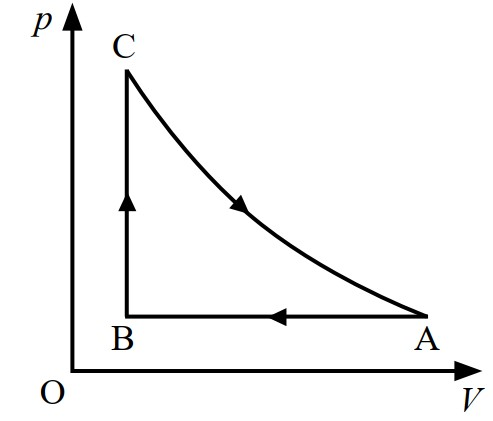
\includegraphics[width=0.5\linewidth]{../figs/G12C2-2}}
	\loigiai{}
\end{ex}
% ===================================================================
\begin{ex}
	 \immini{
	 Một khối khí thực hiện quá trình biến đổi từ trạng thái (1) sang trạng thái (2) như hình bên. Hình nào sau đây biểu diễn đúng quá trình biến đổi của khối khí từ trạng thái (1) sang trạng thái (2) trong hệ tọa độ $(T, p)$?
	 }
	 {
	 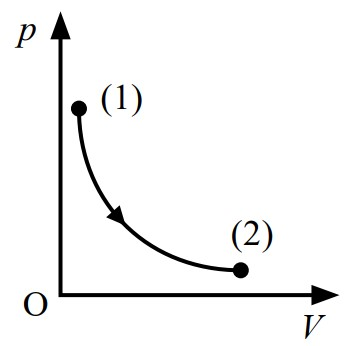
\includegraphics[width=0.4\linewidth]{../figs/G12C2-3}
	 }
	 \begin{center}
	 	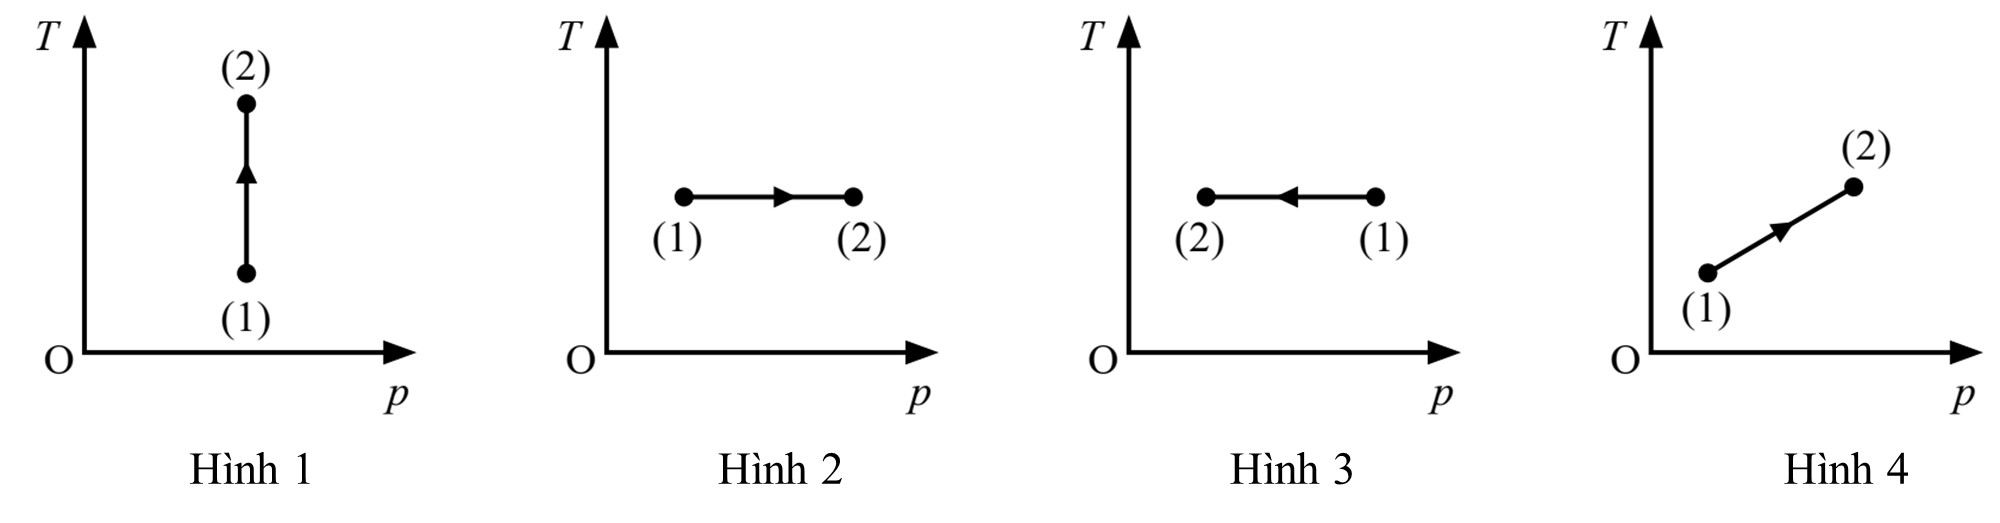
\includegraphics[width=0.8\linewidth]{../figs/G12C2-4}
	 \end{center}
	\choice
	{Hình 1}
	{Hình 2}
	{\True Hình 3}
	{Hình 4}
	\loigiai{}
\end{ex}
% ===================================================================
\begin{ex}
	Một bọt khí tăng gấp đôi bán kính của nó khi nổi từ đáy hồ lên mặt nước. Giả sử bọt khí nổi lên từ từ (nhiệt độ không đổi) và áp suất khí quyển bằng áp suất của một cột nước có độ cao $H$, thì độ sâu của hồ là
	\choice
	{$4 H$}
	{$5 H$}
	{\True $7 H$}
	{$14 H$}
	\loigiai{}
\end{ex}
% ===================================================================
\begin{ex}
	Một quả bóng được bơm đầy khí nitrogen tinh khiết. Quả bóng được xác định có thể tích $\SI{0.75}{\liter}$ vào một ngày có nhiệt độ $\SI{20}{\celsius}$ và áp suất không khí là $\SI{0.85}{atm}$. Có bao nhiêu phân tử nitrogen trong quả bóng?
	\choice
	{\True $1,6 \cdot 10^{22}$}
	{$2,1\cdot10^{20}$}
	{$4,7\cdot10^{23}$}
	{$1,6 \cdot 10^{25}$}
	\loigiai{}
\end{ex}
% ===================================================================
\begin{ex}
	Nén đẳng nhiệt một khối khí lí tưởng xác định làm áp suất khí thay đổi một lượng $\SI{0.5}{atm}$. Biết thể tích và áp suất ban đầu của khối khí là $\SI{5}{\liter}$ và $\SI{2}{atm}$. Thể tích của khối khí lúc sau là
	\choice
	{$\SI{6.25}{\liter}$}
	{\True $\SI{4}{\liter}$}
	{$\SI{6.67}{\liter}$}
	{$\SI{20}{\liter}$}
	\loigiai{\begin{center}
			\begin{tabular}{C{4cm} C{3cm} C{4cm}}
				\colorbox{yellow}{\textcolor{red}{\textbf{Trạng thái 1}}} & $\xrightarrow[]{T_1=T_2}$ & \colorbox{yellow}{\textcolor{red}{\textbf{Trạng thái 2}}}\\
				$p_1=\SI{2}{atm}$ & &$p_2=\SI{2.5}{atm}$\\
				$V_1=\SI{5}{\liter}$ & & $V_2=?$
			\end{tabular}
		\end{center}
		Vì thể tích khí giảm nên áp suất khí tăng.\\
		$$V_2=\dfrac{p_1V_1}{p_2}=\SI{4}{\liter}.$$}
\end{ex}
% ===================================================================
\begin{ex}
	Ở nhiệt độ $\SI{273}{\celsius}$ thể tích của một khối khí lí tưởng là $\SI{10}{\liter}$. Trong điều kiện áp suất không đổi, thể tích của khối khí đó ở nhiệt độ $\SI{546}{\celsius}$ là
	\choice
	{$\SI{20}{\liter}$}
	{\True $\SI{15}{\liter}$}
	{$\SI{12}{\liter}$}
	{$\SI{13.5}{\liter}$}
	\loigiai{\begin{center}
			\begin{tabular}{C{4cm} C{3cm} C{4cm}}
				\colorbox{yellow}{\textcolor{red}{\textbf{Trạng thái 1}}} & $\xrightarrow[]{p_1=p_2}$ & \colorbox{yellow}{\textcolor{red}{\textbf{Trạng thái 2}}}\\
				$V_1=\SI{10}{\liter}$ & &$V_2=?$\\
				$T_1=\SI{546}{\kelvin}$ & & $T_2=\SI{819}{\kelvin}$
			\end{tabular}
		\end{center}
		$$\dfrac{V_1}{T_1}=\dfrac{V_2}{T_2}\Rightarrow V_2=\SI{15}{\liter}.$$}
\end{ex}
% ===================================================================
\begin{ex}
	Một bình chứa khí helium có dung tích $\SI{50}{\liter}$ ở nhiệt độ $\SI{25}{\celsius}$ và áp suất $\SI{20}{atm}$. Người ta muốn dùng khí từ bình này để bơm những quả bóng bay đến dung tích $\SI{2500}{\milli\liter}$ và ở áp suất $\SI{1}{atm}$. Coi nhiệt độ khí là không đổi. Xác định số lượng quả bóng bay có thể bơm được?
	\choice
	{40}
	{120}
	{214}
	{\True 400}
	\loigiai{}
\end{ex}
% ===================================================================
\begin{ex}
	Một khối khí dãn nở đẳng áp có thể tích tăng gấp 1,5 lần thì nhiệt độ của nó tăng thêm $\SI{150}{\celsius}$. Nhiệt độ ban đầu của khối khí là
	\choice
	{$\SI{150}{\celsius}$}
	{$\SI{300}{\celsius}$}
	{$\SI{-123}{\celsius}$}
	{\True $\SI{27}{\celsius}$}
	\loigiai{}
\end{ex}
% ===================================================================
\begin{ex}
	Một khối khí được đựng trong bình kín. Nếu ở $\SI{25}{\celsius}$, áp suất của khí trong bình là $\SI{2}{atm}$ thì ở $\SI{250}{\celsius}$, áp suất của khí là
	\choice
	{$\SI{20}{atm}$}
	{\True $\SI{3.51}{atm}$}
	{$\SI{1.14}{atm}$}
	{$\SI{15.4}{atm}$}
	\loigiai{}
\end{ex}
% ===================================================================
\begin{ex}
	Nén $\SI{10}{\liter}$ khí ở nhiệt độ $\SI{27}{\celsius}$ để cho thể tích của nó chỉ còn $\SI{4}{\liter}$. Trong quá trình nén, nhiệt độ khí tăng $\SI{33}{\celsius}$. So với áp suất ban đầu, áp suất khí lúc sau
	\choice
	{\True tăng 2,775 lần}
	{giảm 2,775 lần}
	{giảm 2,55 lần}
	{tăng 2,55 lần}
	\loigiai{\begin{center}
			\begin{tabular}{C{4cm} C{3cm} C{4cm}}
				\colorbox{yellow}{\textcolor{red}{\textbf{Trạng thái 1}}} & $\xrightarrow[]{\nu=\text{const}}$ & \colorbox{yellow}{\textcolor{red}{\textbf{Trạng thái 2}}}\\
				$p_1$ & &$p_2=?p_1$\\
				$V_1=\SI{10}{\liter}$ & & $V_2=\SI{4}{\liter}$\\
				$T_1=\SI{300}{\kelvin}$ & & $T_2=\SI{333}{\kelvin}$
			\end{tabular}
		\end{center}
		$$\dfrac{p_1V_1}{T_1}=\dfrac{p_2V_2}{T_2}\Rightarrow \dfrac{p_2}{p_1}=\dfrac{V_1}{V_2}\cdot\dfrac{T_2}{T_1}=2,775.$$}
\end{ex}

\Closesolutionfile{ans}
\section{Câu trắc nghiệm đúng sai}
\textit{Thí sinh trả lời từ câu 1 đến câu 4. Trong mỗi ý \textbf{a)}, \textbf{b}, \textbf{c)}, \textbf{d)} ở mỗi câu, thí sinh chọn đúng hoặc sai}
\setcounter{ex}{0}
\Opensolutionfile{ans}[ans/Y24-VN12-PH-C2-TF]
% ===================================================================
\begin{ex}
	Một quả bong bóng được thổi căng, buộc kín miệng rồi đặt vào ngăn mát tủ lạnh.
	\choiceTF[t]
	{Các phân tử khí trong quả bong bóng co lại vì nhiệt độ giảm}
	{\True Các phân tử khí trong quả bong bóng chuyển động chậm hơn}
	{Số lượng phân tử khí trong quả bong bóng giảm}
	{\True Áp suất khí trong quả bong bóng giảm vì các phân tử khí chuyển động chậm hơn và ít va chạm với thành quả bong bóng hơn}
	\loigiai{}
\end{ex}
% ===================================================================
\begin{ex}
	Một khối khí thực hiện các quá trình biến đổi trạng thái như hình bên dưới.
	\begin{center}
		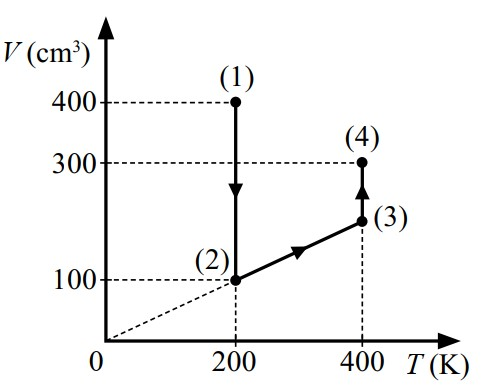
\includegraphics[width=0.35\linewidth]{../figs/G12C2-5}
	\end{center}
	\choiceTF[t]
	{\True $(1)\rightarrow (2)$ là quá trình nén đẳng nhiệt}
	{Áp suất của khối khí ở trạng thái (1) gấp 4 lần áp suất của khối khí ở trạng thái (2)}
	{Áp suất của khối khí ở trạng thái (4) gấp 1,5 lần áp suất của khối khí ở trạng thái (3)}
	{\True Ở trạng thái (2) và (3), khối khí có áp suất lớn nhất}
	\loigiai{}
\end{ex}
% ===================================================================
\begin{ex}
	Một quả bong bóng được thổi căng một phần và thả vào bên trong một chuông thuỷ tinh. Chuông được nối với một máy bơm chân không (hình bên dưới). Không khí trong chuông thuỷ tinh được máy bơm hút dần ra ngoài. Xem nhiệt độ của khí là không đổi.
	\begin{center}
		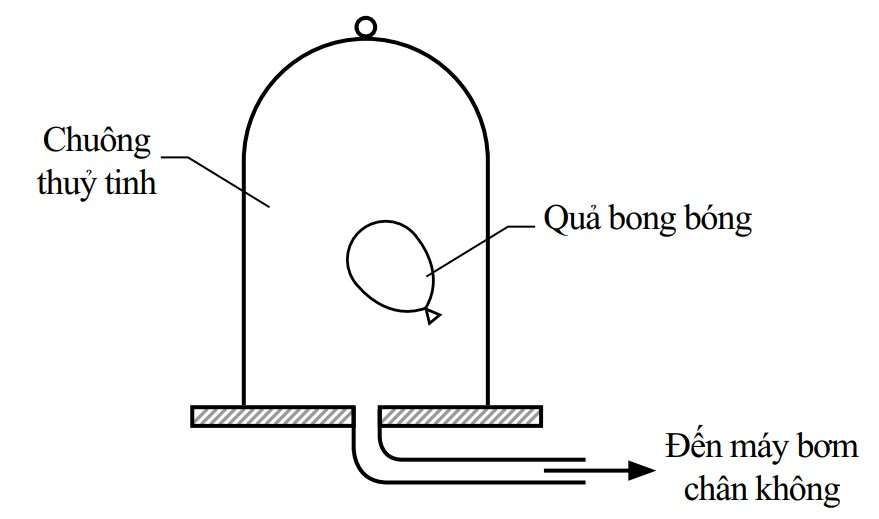
\includegraphics[width=0.4\linewidth]{../figs/G12C2-6}
	\end{center}
	\choiceTF[t]
	{\True Khi không khí được bơm dần ra ngoài thì áp suất không khí bên trong chuông giảm}
	{\True Khi không khí được bơm dần ra ngoài thì quả bong bóng dần căng phồng lên}
	{Quá trình căng phồng của quả bong bóng là quá trình dãn nở đẳng áp}
	{\True Khi quả bong bóng căng phồng lên, thể tích không khí bên trong quả bong bóng tăng lên và áp suất không khí bên trong quả bong bóng giảm}
	\loigiai{}
\end{ex}
% ===================================================================
\begin{ex}
	Một bình kín chứa $\SI{50}{\liter}$ khí oxygen ở $\SI{15}{\celsius}$ và áp suất $\SI{2.5E5}{\pascal}$.
	\choiceTF[t]
	{Lượng khí oxygen trong bình là $\SI{2.5}{\mole}$}
	{\True Thể tích của lượng khí trên ở điều kiện tiêu chuẩn xấp xỉ $\SI{117}{\liter}$}
	{\True Nếu đem bình ra phơi nắng để nhiệt độ khí trong bình tăng lên đến $\SI{49}{\celsius}$ thì áp suất khí trong bình khi đó xấp xỉ $\SI{2.8E5}{\pascal}$ (bỏ qua sự dãn nở vì nhiệt của bình chứa)}
	{Nếu mang bình đang đặt ngoài nắng vào trong nhà thì tốc độ chuyển động nhiệt của các phân tử khí trong bình tăng lên}
	\loigiai{}
\end{ex}
\Closesolutionfile{ans}
\section{Câu trắc nghiệm trả lời ngắn} \textit{Thí sinh trả lời từ câu 1 đến câu 6}
\setcounter{ex}{0}
% ===============================================================
\begin{ex}
	Một lượng khí lí tưởng thực hiện bốn quá trình như hình bên.
	Trong quá trình nào, áp suất của khí không đổi?
\begin{center}
	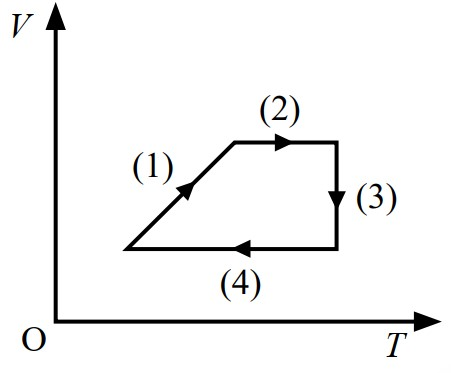
\includegraphics[width=0.25\linewidth]{../figs/G12C2-9}
\end{center}
	
	\shortans{1}
	\loigiai{
		
	}
\end{ex}
\Opensolutionfile{ans}[ans/Y24-VN12-PH-C2-TL]
% ===============================================================
\begin{ex}
	Khi đun nóng đẳng tích một khối khí thêm $\SI{1}{\celsius}$ thì áp suất khối khí tăng thêm $\dfrac{1}{360}$	áp suất ban đầu. Nhiệt độ ban đầu của khối khí đó là bao nhiêu $\si{\celsius}$?
	\shortans{87}
	\loigiai{
		$$\dfrac{p}{t+273}=\dfrac{p\left(1+\dfrac{1}{360}\right)}{t+274}\Rightarrow t=\SI{87}{\celsius}.$$
	}
\end{ex}
% ===============================================================
\begin{ex}
	Một bình có dung tích $\SI{4}{\liter}$ chứa một khối khí ở áp suất $\SI{2.4}{atm}$. Bình này được nối thông với một bình thứ hai có dung tích $\SI{8}{\liter}$ và được hút chân không. Xem nhiệt độ không đổi. Áp suất của khối khí sau khi hai bình được nối thông với nhau là bao nhiêu (tính theo đơn vị $\si{atm}$)?
	\shortans{0,8}
	\loigiai{
		$$p_1V_1=p_2\left(V_1+V_2\right)\Rightarrow p_2=\dfrac{2,4\cdot4}{12}=\SI{0.8}{atm}.$$
	}
\end{ex}
% ===============================================================
\begin{ex}
	Một lượng khí được chứa trong một xilanh được đậy kín bởi một pit-tông động như hình bên dưới. Ban đầu, độ dài phần xilanh chứa khí là $\SI{100}{\centi\meter}$, nhiệt độ khí là $\SI{27}{\celsius}$. Khi lượng khí được đun nóng đều thì pit-tông từ từ dịch chuyển cho đến khi độ dài phần xilanh chứa khí là $\SI{120}{\centi\meter}$. Nhiệt độ khí khi đó là bao nhiêu (tính theo đơn vị $\si{\celsius}$)?
	\begin{center}
		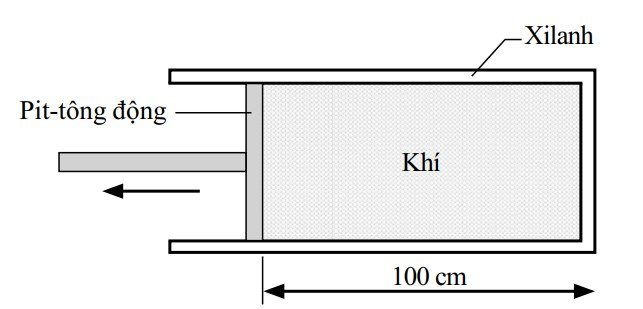
\includegraphics[width=0.4\linewidth]{../figs/G12C2-7}
	\end{center}
	\shortans{87}
	\loigiai{
		$$\dfrac{\ell_0S}{T_0}=\dfrac{\ell S}{T}\Leftrightarrow \dfrac{100}{27+273}=\dfrac{120}{t+273}\Rightarrow t=\SI{87}{\celsius}.$$
	}
\end{ex}
% ===============================================================
\begin{ex}
	Một khối khí thực hiện các quá trình biến đổi trạng thái như hình bên. Ở trạng thái (1), khối khí chiếm thể tích
	$\SI{1.2}{\liter}$. Xác định thể tích của khối khí ở trạng thái (3) (theo đơn vị $\si{\liter}$).
	\begin{center}
		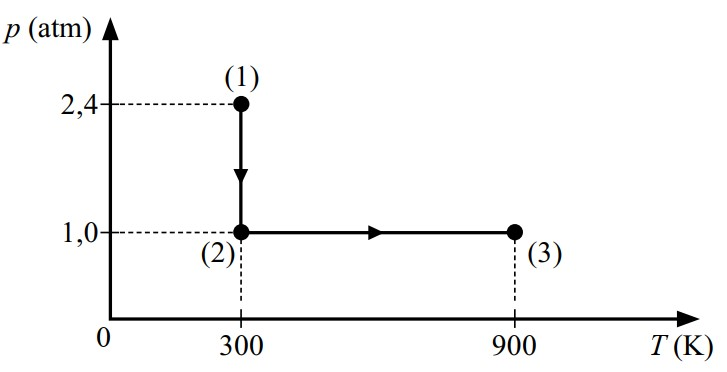
\includegraphics[width=0.4\linewidth]{../figs/G12C2-8}
	\end{center}
	\shortans{8,64}
	\loigiai{
	$$\dfrac{p_1V_1}{T_1}=\dfrac{p_2V_2}{T_2}\Leftrightarrow \dfrac{2,4\cdot1,2}{300}=\dfrac{1,0\cdot V_3}{900}\Rightarrow V_3=\SI{8.64}{\liter}.$$
	}
\end{ex}
%% ===============================================================
%\begin{ex}
%	Một khối khí chứa trong một bình đậy kín bằng một pit-tông động. Nhiệt độ và áp suất của khối khí lần lượt là $\SI{30}{\celsius}$ và $\SI{2.5E5}{\pascal}$. Pit-tông từ từ nén khối khí để thể tích khối khí giảm còn $\SI{10}{\percent}$ thể tích ban đầu thì thấy áp suất khối khí tăng lên đến $\SI{5.0E6}{\pascal}$. Nhiệt độ của khối khí biến thiên một lượng bao nhiêu $\si{\celsius}$?
%	\shortans{2.38}
%	\loigiai{
%		2.38
%	}
%\end{ex}
% ===============================================================
\begin{ex}
	Ở độ cao $h$, không khí có áp suất $\SI{230}{\milli\meter Hg}$ và nhiệt độ $\SI{-43}{\celsius}$. Xác định khối lượng riêng của không khí ở độ cao $h$ (theo đơn vị $\si{\kilogram/\meter^3}$, kết quả làm tròn đến hai chữ số
	thập phân). Giả sử ở mặt đất không khí có áp suất $\SI{760}{\milli\meter Hg}$, khối lượng riêng $\SI{1.22}{\kilogram/\meter^3}$,
	nhiệt độ $\SI{15}{\celsius}$.
	\shortans{0,46}
	\loigiai{
	$$\dfrac{D_2}{D_1}=\dfrac{V_1}{V_2}=\dfrac{p_2}{p_1}\cdot\dfrac{T_1}{T_2}\Rightarrow D_2=1,22\cdot\dfrac{230}{760}\cdot\left(\dfrac{15+273}{-43+273}\right)\approx\SI{0.46}{\kilogram/\meter^3}.$$
	}
\end{ex}
\Closesolutionfile{ans}